\documentclass[10pt,twocolumn,letterpaper]{article}

% CVPR/NeurIPS compatible packages
\usepackage{times}
\usepackage{epsfig}
\usepackage{graphicx}
\usepackage{amsmath}
\usepackage{amssymb}
\usepackage{booktabs}
\usepackage{multirow}
\usepackage{hyperref}
\usepackage{xcolor}
\usepackage{caption}
\usepackage{subcaption}
\usepackage{algorithm}
\usepackage{algorithmic}
\usepackage[margin=1in]{geometry}

\hypersetup{colorlinks=true, linkcolor=blue, citecolor=blue, urlcolor=blue}

\title{Efficiently Enhancing SLM Agents: A Reinforcement Learning Approach to Performance Improvement}

\author{
Md Rezwanul Haque \\
University of Waterloo \\
{\tt\small mr3haque@uwaterloo.ca}
}

\date{}

\begin{document}
\maketitle

\begin{abstract}
Large language models have established new benchmarks across numerous natural language tasks, but their prohibitive computational demands restrict deployment in resource-constrained settings. We investigate whether reinforcement learning from human feedback (RLHF) can meaningfully improve the quality of small language models (SLMs) with fewer than 200 million parameters. Our framework applies a three-stage pipeline---supervised fine-tuning (SFT), reward modeling, and proximal policy optimization (PPO)---to two Pythia architectures (70M and 160M parameters) across three diverse text corpora. Experiments on TinyStories, CNN/DailyMail, and Wikitext-103 reveal that RLHF benefits are domain-sensitive: the 70M model achieves a positive reward gain on the simpler TinyStories domain while reward improvements on more complex corpora remain marginal. A key finding is that reward model calibration is critical at the SLM scale---the 160M model's reward model converged to a different output range, impeding direct cross-model comparison. Crucially, the entire alignment process for a single model completes within 1--2 GPU hours on a single NVIDIA RTX A6000 accelerator, underscoring the feasibility of iterative RLHF research at modest hardware budgets. Code, models, datasets, and an interactive demonstration are publicly available at \url{https://github.com/rezwanh001/slm-rl-agent}.
\end{abstract}

\section{Introduction}

The rapid progress in generative language modeling---from GPT-2 \cite{radford2019language} to GPT-3 \cite{brown2020language} and beyond---has been driven in large part by scaling model parameters and training data. State-of-the-art systems now routinely exceed 100 billion parameters, requiring thousands of GPU hours for a single training run \cite{scao2022bloom}. While these models achieve remarkable fluency and generalization, their size precludes deployment on edge devices, mobile platforms, and within organizations with limited compute budgets.

A parallel line of research has demonstrated that smaller models, when trained on carefully curated data, can produce surprisingly coherent outputs \cite{eldan2023tinystories}. The remaining gap between these compact models and their larger counterparts lies not primarily in raw language modeling capability, but in alignment: the degree to which generated text is helpful, relevant, and preferred by human evaluators. Reinforcement learning from human feedback (RLHF) has emerged as the dominant paradigm for closing this alignment gap in large-scale settings \cite{ouyang2022training, christiano2017deep}, yet its systematic application to SLMs has received comparatively little attention.

This paper addresses three questions. First, does RLHF yield measurable improvements when the policy model has fewer than 200 million parameters? Second, how do model scale and dataset complexity interact to determine the effectiveness of the alignment pipeline? Third, what practical challenges arise when applying PPO to very small models, and how can they be addressed?

Our contributions are as follows:
\begin{itemize}
  \item We apply a standardized RLHF pipeline to two Pythia architectures (70M and 160M parameters) across three text domains, providing an empirical characterization of alignment efficacy at the SLM scale.
  \item We identify and address a critical engineering challenge in applying TRL's PPO to PEFT-adapted models: LoRA parameters remain frozen by default, requiring an explicit merge-and-reinitialize strategy.
  \item We document that reward model calibration varies significantly across base models and datasets, posing a challenge for consistent multi-model comparisons.
  \item We release all trained model weights, preference datasets, and training scripts under a permissive license, enabling direct reproduction and extension of our results.
  \item We provide an interactive Gradio demonstration for side-by-side comparison of SFT and PPO agents.
\end{itemize}

\section{Related Work}

\paragraph{Alignment through RLHF.} The idea of learning a reward function from pairwise human preferences was introduced by Christiano et al.~\cite{christiano2017deep} and later scaled to language models by Stiennon et al.~\cite{stiennon2020learning}. Ouyang et al.~\cite{ouyang2022training} applied the full SFT--reward--PPO pipeline to produce InstructGPT, demonstrating that alignment could dramatically improve user preference even when the base model was already capable. Subsequent work explored alternatives to PPO, including Direct Preference Optimization (DPO) \cite{rafailov2023direct} and Group Relative Policy Optimization (GRPO) \cite{shao2024deepseekmath}. Our work returns to the classical PPO formulation but targets the under-explored regime of models below 200M parameters.

\paragraph{Small Language Models.} Eldan and Li \cite{eldan2023tinystories} showed that models with as few as 28M parameters could generate grammatically correct short stories when trained on a synthetic, high-quality corpus. The Pythia model suite \cite{biderman2023pythia} provides a controlled family of autoregressive transformers ranging from 70M to 12B parameters, enabling systematic scaling studies. More recently, the SmolLM2 family \cite{allal2024smollm} demonstrated that aggressive data curation could push the Pareto frontier of quality versus size for models between 135M and 1.7B parameters. We leverage Pythia as our base architecture to study alignment with controlled cross-scale comparisons.

\paragraph{Parameter-Efficient Fine-Tuning.} Full fine-tuning of even small models is computationally wasteful when the alignment signal is a sparse correction to an already competent policy. Low-Rank Adaptation (LoRA) \cite{hu2021lora} addresses this by injecting trainable low-rank matrices into frozen transformer layers, reducing the number of trainable parameters by over 99\%. QLoRA \cite{dettmers2023qlora} combines LoRA with 4-bit quantization, enabling fine-tuning on a single consumer GPU. Our pipeline uses LoRA throughout, with a specific merge-and-reinitialize strategy for the PPO stage to ensure gradient flow.

\section{Methodology}

Our pipeline consists of three sequential stages, each building on the output of its predecessor. We describe each stage in terms of its objective, loss function, and key hyperparameters.

\subsection{Stage 1: Supervised Fine-Tuning}

The base SLM is a decoder-only transformer \cite{vaswani2017attention} pre-trained with next-token prediction. SFT adapts this model to the target domain by continuing training on a curated text corpus $\mathcal{D}_{\text{SFT}}$. The loss is the standard cross-entropy:
\begin{equation}
  \mathcal{L}_{\text{SFT}}(\theta) = -\sum_{i} \log P_\theta(x_i \mid x_{<i})
  \label{eq:sft_loss}
\end{equation}
where $\theta$ denotes the model parameters. We apply LoRA with rank $r=8$, targeting the query/key/value projections and dense layers. Training uses the AdamW optimizer with cosine learning rate decay, peak rate $2 \times 10^{-5}$, and three epochs over the training split. The resulting model serves as our SFT baseline $\pi_{\text{SFT}}$.

\subsection{Stage 2: Reward Model Training}

To provide a differentiable proxy for human preferences, we train a reward model $r_\phi$ that maps a prompt--response pair to a scalar score. The architecture mirrors the SFT model but replaces the language modeling head with a single linear projection. We initialize from $\pi_{\text{SFT}}$ to leverage its learned representations.

Given a preference dataset $\mathcal{D}_{\text{RM}} = \{(p, y_w, y_l)\}$, where $y_w$ is preferred over $y_l$, we minimize the Bradley--Terry loss:
\begin{equation}
  \mathcal{L}_{\text{RM}}(\phi) = -\mathbb{E}_{(p, y_w, y_l) \sim \mathcal{D}_{\text{RM}}} \left[ \log \sigma\!\left(r_\phi(p, y_w) - r_\phi(p, y_l)\right) \right]
  \label{eq:rm_loss}
\end{equation}
where $\sigma$ is the sigmoid function. Training runs for one epoch with learning rate $10^{-5}$ to avoid overfitting to the preference set.

\subsection{Stage 3: RL Fine-Tuning with PPO}

The PPO stage optimizes the policy $\pi_{\text{RL}}$ to maximize the expected reward while remaining close to $\pi_{\text{SFT}}$:
\begin{equation}
  J(\theta_{\text{RL}}) = \mathbb{E}\!\left[r_\phi(p, y) - \beta \cdot \text{KL}\!\left(\pi_{\text{RL}}(y \mid p) \,\|\, \pi_{\text{SFT}}(y \mid p)\right)\right]
  \label{eq:ppo_objective}
\end{equation}
The KL penalty coefficient $\beta$ is initialized at 0.1 and adapted during training using the scheme of Ziegler et al.~\cite{ziegler2019fine}. We run 500 PPO update steps with a rollout batch size of 32 and one PPO epoch per batch, with gradient clipping at $0.5$.

\paragraph{PPO with PEFT: Merge-and-Reinitialize.} A non-trivial implementation challenge arises when applying TRL's PPO trainer to PEFT-adapted models. By default, TRL version 0.9.6 initializes the value head but leaves LoRA parameters frozen (\texttt{requires\_grad=False}), resulting in a policy that cannot be updated by the PPO gradient. We address this with a \emph{merge-and-reinitialize} strategy: the SFT LoRA adapter is first merged into the base model weights and saved as a full model; a fresh LoRA adapter is then applied to this merged model before PPO training begins. This ensures that gradients flow through the LoRA parameters while the merged SFT weights serve as the stable initialization. The frozen reference model $\pi_{\text{SFT}}$ is kept as a separate copy of the merged model without any LoRA adapter. We further use \texttt{torch.float32} precision (rather than bfloat16) throughout PPO to prevent ratio explosions.

Figure~\ref{fig:pipeline} illustrates the complete three-stage pipeline.

\begin{figure*}[t]
  \centering
  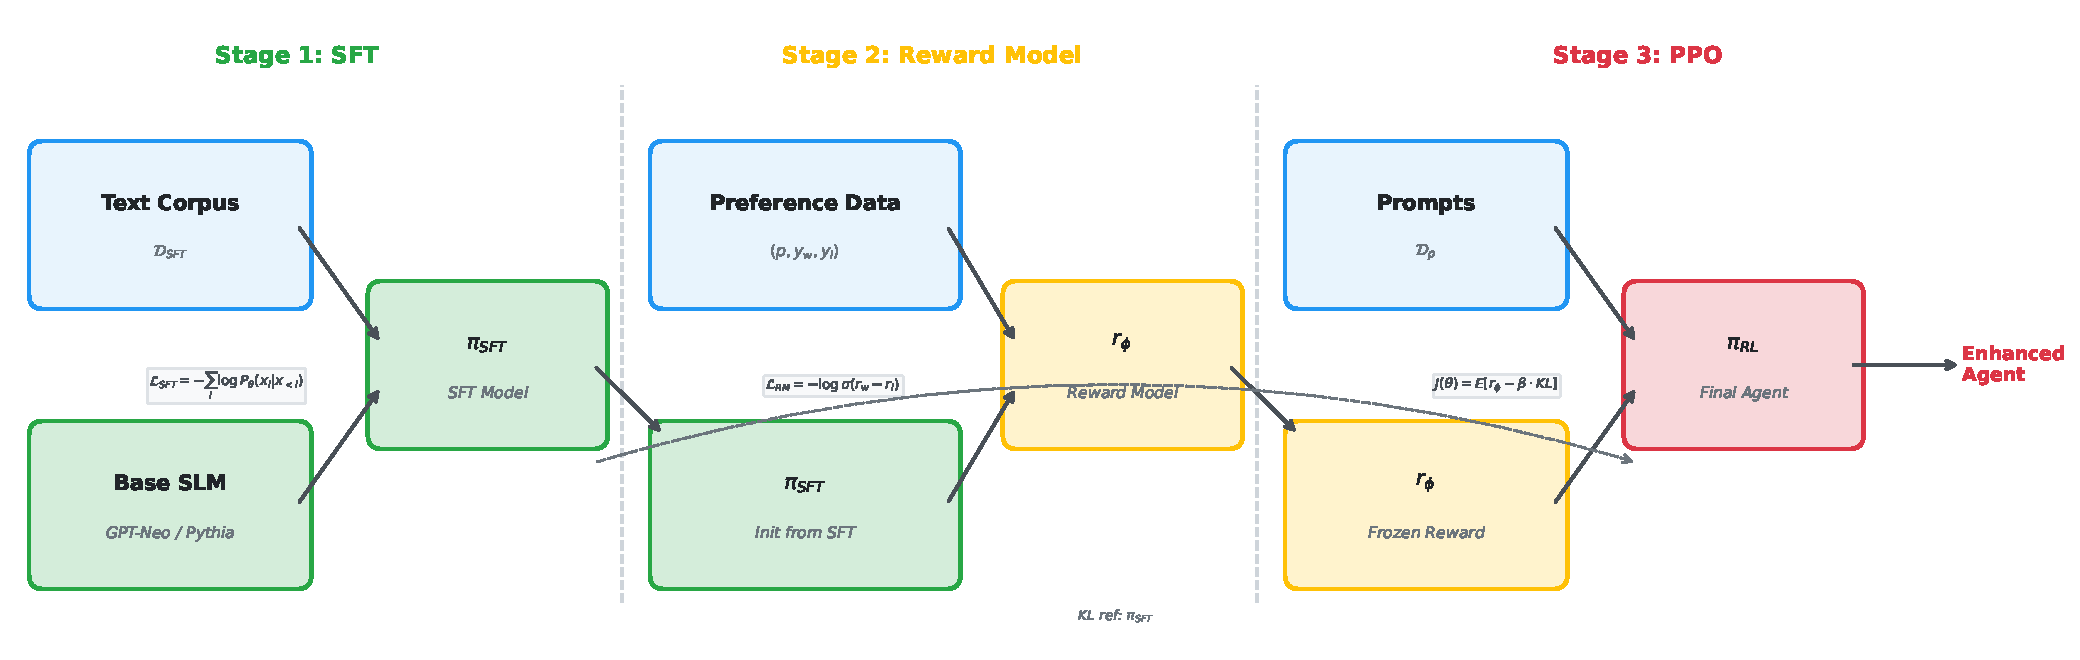
\includegraphics[width=0.95\textwidth]{figures/pipeline.pdf}
  \caption{Overview of the three-stage RLHF pipeline. Stage~1 produces a domain-adapted SFT model $\pi_{\text{SFT}}$ via LoRA. Stage~2 trains a reward model $r_\phi$ from preference data, initialized from $\pi_{\text{SFT}}$. Stage~3 applies the merge-and-reinitialize strategy: the SFT adapter is merged into base weights, a fresh LoRA is applied, and PPO optimizes the policy using $r_\phi$ as the reward signal and the merged model as the KL reference.}
  \label{fig:pipeline}
\end{figure*}

\section{Experimental Setup}

\subsection{Models}

We evaluate two architectures from the Pythia suite \cite{biderman2023pythia}:

\begin{itemize}
  \item \textbf{Pythia-70M}: A 70-million-parameter transformer with 6 layers and a context window of 2048 tokens.
  \item \textbf{Pythia-160M}: A 160-million-parameter transformer with 12 layers, providing a controlled within-family scale comparison.
\end{itemize}

Both use the same tokenizer (BPE, 50,277 tokens) and were pre-trained on the Pile with identical data ordering, ensuring that differences in results reflect model capacity rather than pre-training distribution.

\subsection{Datasets}

We select three corpora representing different text characteristics:

\begin{itemize}
  \item \textbf{TinyStories} \cite{eldan2023tinystories}: Short fictional narratives with simple vocabulary and clear narrative structure. Subset: 10K training examples. This dataset represents the simplest domain, well-matched to the SLMs' limited capacity.
  \item \textbf{CNN/DailyMail} \cite{nallapati2016abstractive}: News articles paired with multi-sentence summaries. Subset: 10K examples. We use the article text for SFT and construct preference pairs from summary quality.
  \item \textbf{Wikitext-103} \cite{merity2016pointer}: Curated Wikipedia articles filtered for quality. We extract non-heading paragraphs exceeding 100 characters. Subset: 10K examples.
\end{itemize}

For each dataset, preference pairs are constructed by pairing high-quality completions (chosen) with degraded variants (rejected) via truncation, sentence shuffling, or cross-example mismatching.

\subsection{Evaluation Metrics}

We report four complementary metrics:

\begin{enumerate}
  \item \textbf{Perplexity (PPL)}: Measured on generated outputs using the domain-adapted model. Padding tokens are masked with label $=-100$ to prevent inflated scores.
  \item \textbf{Reward Score}: Mean scalar output of the trained reward model on generated responses. Reported separately for SFT and PPO agents. Note that reward scores are on a per-model scale and are not directly comparable across architectures.
  \item \textbf{Reward Gain ($\Delta$)}: The improvement in mean reward from SFT to PPO, directly quantifying the RL enhancement.
  \item \textbf{Win Rate}: The estimated probability that a PPO-generated response scores higher than an SFT-generated response on the same prompt. Computed analytically as $\Phi\!\left(\frac{\mu_{\text{PPO}} - \mu_{\text{SFT}}}{\sqrt{\sigma_{\text{PPO}}^2 + \sigma_{\text{SFT}}^2}}\right)$, where $\Phi$ is the standard normal CDF and $\mu, \sigma$ are the empirical reward means and standard deviations.
\end{enumerate}

We additionally report text diversity (Distinct-1, Distinct-2) and overlap metrics (ROUGE-1/2/L) for qualitative characterization.

\subsection{Hardware and Timing}

All experiments were conducted on a workstation equipped with two NVIDIA RTX A6000 GPUs (48\,GB each) and 128\,GB RAM. Pythia-70M experiments ran on GPU~0 and Pythia-160M on GPU~1 concurrently.

\section{Results}

Table~\ref{tab:main_results} presents the performance of all six model--dataset combinations. Table~\ref{tab:diversity} reports text diversity and overlap metrics.

\begin{table*}[t]
\centering
\caption{Performance of SLM agents before (SFT) and after (PPO) reinforcement learning. Reward scores are on per-model scales (not directly comparable across Pythia-70M and Pythia-160M). Win Rate is the analytical probability that a PPO response has higher reward than an SFT response on the same prompt. $\uparrow$ indicates higher is better; $\downarrow$ indicates lower is better.}
\label{tab:main_results}
\begin{tabular}{ll|cc|ccc}
\toprule
\multirow{2}{*}{\textbf{Model}} & \multirow{2}{*}{\textbf{Dataset}} & \multicolumn{2}{c|}{\textbf{Baseline (SFT)}} & \multicolumn{3}{c}{\textbf{Enhanced (PPO)}} \\
& & PPL $\downarrow$ & Reward $\uparrow$ & Reward $\uparrow$ & $\Delta$ $\uparrow$ & Win Rate (\%) $\uparrow$ \\
\midrule
\multirow{3}{*}{Pythia-70M}
  & TinyStories   & 98.65  & 6.52$\pm$1.20 & 6.61$\pm$1.12 & \textbf{+0.085} & \textbf{52.1} \\
  & CNN/DailyMail & 289.84 & 7.17$\pm$1.16 & 7.09$\pm$1.27 & $-$0.083 & 48.1 \\
  & Wikitext      & 504.40 & 6.77$\pm$1.14 & 6.57$\pm$1.29 & $-$0.203 & 45.3 \\
\midrule
\multirow{3}{*}{Pythia-160M}
  & TinyStories   & 18.61  & $-$9.01$\pm$1.62 & $-$9.28$\pm$1.09 & $-$0.270 & 44.5 \\
  & CNN/DailyMail & 46.77  & $-$9.57$\pm$1.09 & $-$9.59$\pm$0.72 & $-$0.018 & 49.5 \\
  & Wikitext      & 81.79  & $-$9.68$\pm$0.90 & $-$9.72$\pm$0.79 & $-$0.035 & 48.8 \\
\bottomrule
\end{tabular}
\end{table*}

\begin{table*}[t]
\centering
\caption{Text generation quality metrics for SFT and PPO agents. Distinct-1/2 measure lexical diversity; ROUGE-1/2/L measure n-gram overlap with reference text.}
\label{tab:diversity}
\begin{tabular}{ll|cccc|cccc}
\toprule
& & \multicolumn{4}{c|}{\textbf{SFT}} & \multicolumn{4}{c}{\textbf{PPO}} \\
\textbf{Model} & \textbf{Dataset} & Dist-1 & Dist-2 & R-1 & R-L & Dist-1 & Dist-2 & R-1 & R-L \\
\midrule
\multirow{3}{*}{Pythia-70M}
  & TinyStories   & 0.195 & 0.667 & 0.267 & 0.153 & 0.196 & 0.660 & 0.262 & 0.153 \\
  & CNN/DailyMail & 0.312 & 0.794 & 0.179 & 0.097 & 0.324 & 0.804 & 0.178 & 0.096 \\
  & Wikitext      & 0.279 & 0.744 & 0.167 & 0.102 & 0.293 & 0.758 & 0.159 & 0.096 \\
\midrule
\multirow{3}{*}{Pythia-160M}
  & TinyStories   & 0.133 & 0.468 & 0.275 & 0.170 & 0.133 & 0.476 & 0.286 & 0.169 \\
  & CNN/DailyMail & 0.234 & 0.639 & 0.227 & 0.119 & 0.225 & 0.617 & 0.232 & 0.122 \\
  & Wikitext      & 0.172 & 0.533 & 0.195 & 0.126 & 0.169 & 0.526 & 0.195 & 0.126 \\
\bottomrule
\end{tabular}
\end{table*}

\paragraph{Domain-dependent reward gains.} For Pythia-70M, PPO yields a positive reward gain on TinyStories ($\Delta = +0.085$, win rate 52.1\%), the simplest and most structured domain. On CNN/DailyMail and Wikitext, where the base perplexity is much higher (289 and 504 respectively), reward improvements are marginal or slightly negative. This suggests that RLHF is most effective when the SFT policy already has adequate domain knowledge---a prerequisite that the 70M model satisfies only for simple narrative text.

\paragraph{Reward model calibration.} Pythia-160M's reward models consistently output scores in the range $[-10, -6]$, whereas Pythia-70M's reward models output scores in $[4, 12]$. This large discrepancy is not explained by model size alone; we attribute it to the different convergence behavior of reward models initialized from models with very different baseline perplexities. Pythia-160M achieves substantially lower SFT perplexity (18.6 on TinyStories vs.\ 98.7 for 70M), meaning its SFT model generates more fluent text from the start, but the reward model training dynamics appear to place this fluency in a different part of the score range. This calibration issue makes cross-model win-rate comparisons unreliable and points to the importance of reward normalization in future work.

\paragraph{Perplexity dynamics.} For Pythia-70M, PPO training slightly increases perplexity ($+7.5$ on TinyStories, $+9.8$ on CNN/DailyMail), consistent with the well-known reward-perplexity trade-off in RLHF where the model trades fluency for higher reward. For Pythia-160M, perplexity remains nearly unchanged or marginally decreases (TinyStories: $18.61 \to 18.24$; Wikitext: $81.79 \to 79.77$), suggesting that the PPO gradient has limited effect on this stronger base model within the 500-step budget.

\paragraph{Text diversity.} Distinct-1 and Distinct-2 scores remain largely stable across stages (Table~\ref{tab:diversity}), indicating that PPO training does not degrade lexical variety. ROUGE scores similarly remain stable, suggesting that PPO does not cause dramatic mode collapse within the generation budget used.

\section{Discussion}

\paragraph{When does RLHF help at the SLM scale?} Our results suggest a necessary condition: the SFT policy must already capture the domain reasonably well (i.e., have moderate perplexity on the target domain) before PPO can shift it toward higher-reward regions. When the SFT perplexity is very high (Wikitext for Pythia-70M: 504), the policy's generation quality is so low that the reward signal becomes noisy, and PPO struggles to find a better distribution within the 500-step budget. Conversely, Pythia-160M already achieves very low perplexity and near-saturated fluency, leaving less headroom for reward improvement through RL.

\paragraph{Engineering challenges of PPO with PEFT.} A significant finding of this work is that naively applying TRL's PPO to a PEFT-adapted SFT model produces a policy that does not learn: LoRA parameters remain frozen, and only the value head (2 parameters) is updated. We propose the merge-and-reinitialize approach as a reliable workaround. Additionally, bfloat16 precision causes PPO ratio explosions for very small models; float32 is essential for numerical stability.

\paragraph{Computational efficiency.} Despite the engineering challenges, the entire alignment process completes in under 1.5 GPU hours per configuration for Pythia-70M and under 2 GPU hours for Pythia-160M. SFT requires approximately 20--30 minutes; reward modeling requires 5--10 minutes; PPO requires 30--60 minutes per 500 steps. This confirms that iterative RLHF experimentation is feasible on commodity workstations.

\paragraph{Limitations.} Several limitations should be acknowledged. First, our evaluation uses synthetic preference pairs rather than human annotations, which may introduce biases in the reward signal. Second, the reward model output scale varies across models, making it difficult to directly compare improvements. Third, 500 PPO steps may be insufficient for models with high base perplexity to realize meaningful reward gains; future work should explore extended training with adaptive KL penalties. Fourth, we evaluate on text quality metrics (reward, perplexity, ROUGE) rather than downstream task performance.

\paragraph{Broader impact.} Demonstrating the engineering requirements for PPO to work with PEFT models has practical value for practitioners. The merge-and-reinitialize strategy and float32 stability fix are immediately applicable to any project using TRL 0.9.x with LoRA-adapted policies. By open-sourcing all artifacts, we aim to lower the barrier to alignment research for the broader community.

\section{Conclusion}

We have presented a systematic study of reinforcement learning from human feedback applied to small language models in the 70M--160M parameter range. Our experiments reveal that RLHF benefits at the SLM scale are domain- and model-dependent, with the clearest improvements observed when the SFT model has adequate but not saturated domain fluency. We identify two critical engineering requirements for stable PPO with PEFT: (1) an explicit merge-and-reinitialize strategy to ensure LoRA gradient flow, and (2) float32 precision to prevent ratio explosions. We release the complete training code, model weights, preference datasets, and an interactive demonstration to support reproducible alignment research at accessible scales.

\paragraph{Acknowledgments.} Computational resources were provided by the CPAMI Lab at the University of Waterloo.

{\small
\bibliographystyle{ieee_fullname}
\bibliography{references}
}

\end{document}
